% !TeX spellcheck = en_US
\section{Procedure}
In every experiment we measured the temperature of the liquid.

\subsection{Falling Sphere Viscometer}

The experiment setup is shown in Figure~\ref{fig:kug}.

We measured the time it takes a sphere to fall the distance between the first and the second mark. The sphere should have reached its terminal velocity when it passes the first mark. The second mark is above the bottom of the cylinder in order to assure the validity of formula~\ref{eq:term}. This measurement was performed ten times with identical spheres of known mass and radius. Both of us measured the time independently but $5$ out of the $20$ measurements had to be discarded for different reasons%
\footnote{mostly because we didn't press the button on the stopwatch quick enough}%
.
Finally we measured the density of the liquid using an areometer.

\subsection{Capillary Viscometer}

The experiment setup is shown in Figure \ref{fig:cap}.

We let the water flow through the cannula for $\unit[100]{s}$ an weigh the amount of water that flowed through it. Since the diameter of the hose is significantly larger than that of the cannula we can neglect it for our calculations. The height difference between the cannula and the water line of the reservoir was varied five times each for two different cannulae. 

\subsection{Ubbelohde Viscometer}

The experiment setup is shown in Figure \ref{fig:ubb}.

The upper vessel of this apparatus was filled with water above the upper mark. Then we measured the time between the moment in which the water level passed the first mark and the moment it passed the second mark. We performed a total of five independent measurements.



\begin{figure}
    \begin{minipage}{.3\textwidth}
        \centering
        \vspace{4.mm}
        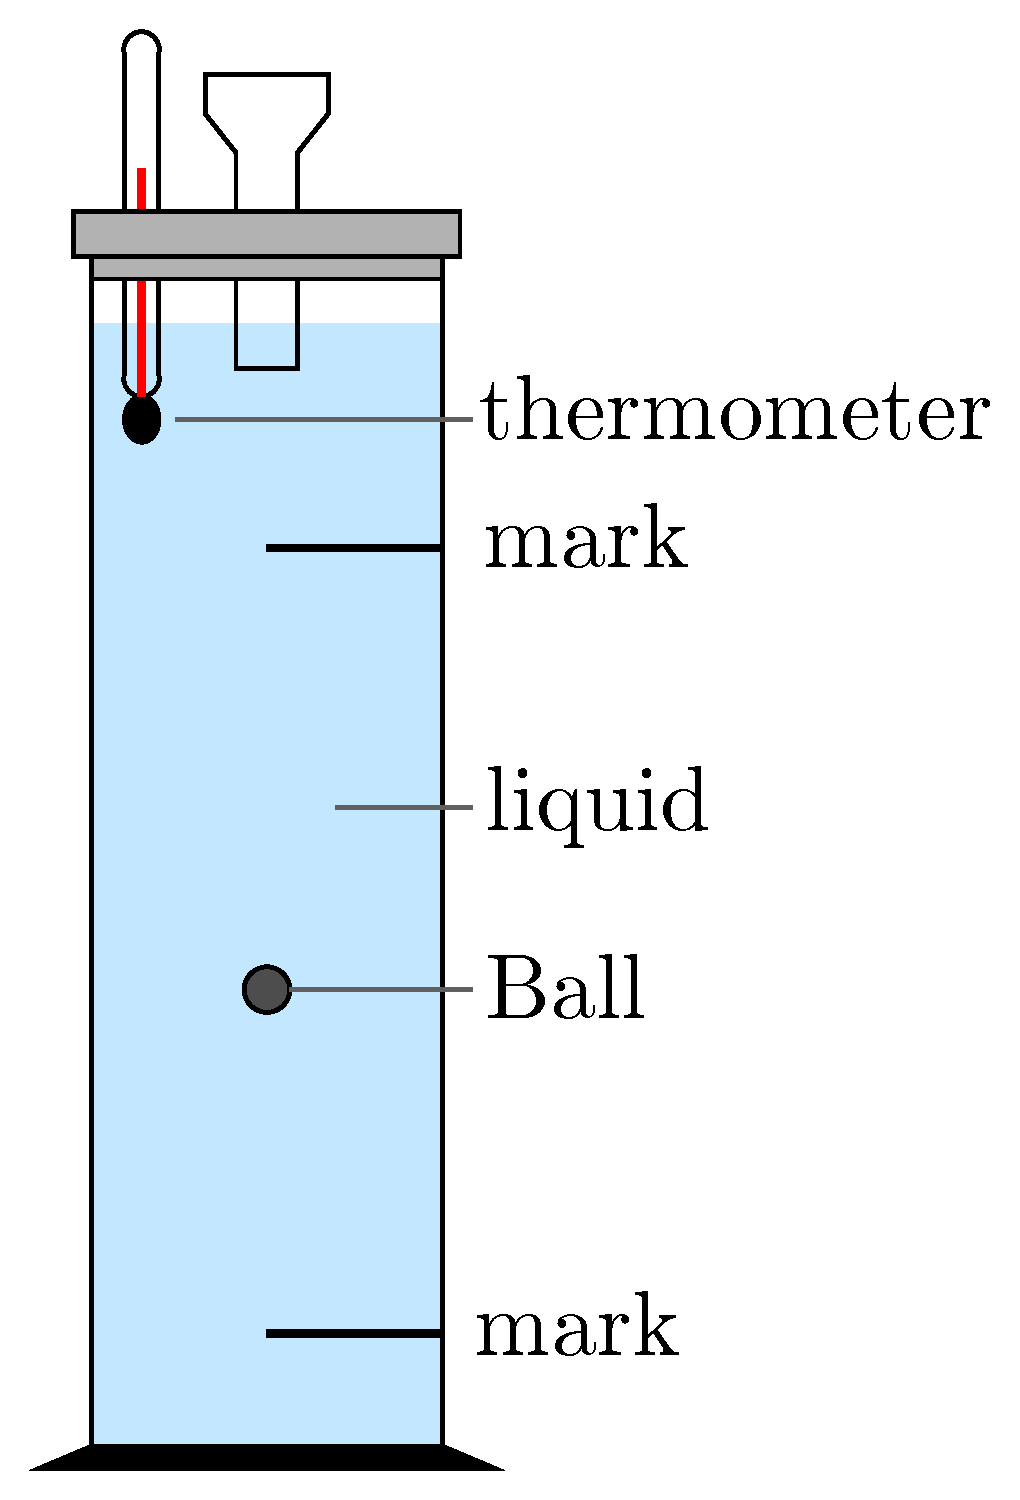
\includegraphics[scale=.25]{Bilder/kugelfall.pdf}
        \vspace{4.mm}
        \caption{falling sphere viscometer}
        \label{fig:kug}
    \end{minipage}
    \hspace{5mm}
    \begin{minipage}{.3\textwidth}
    \centering
    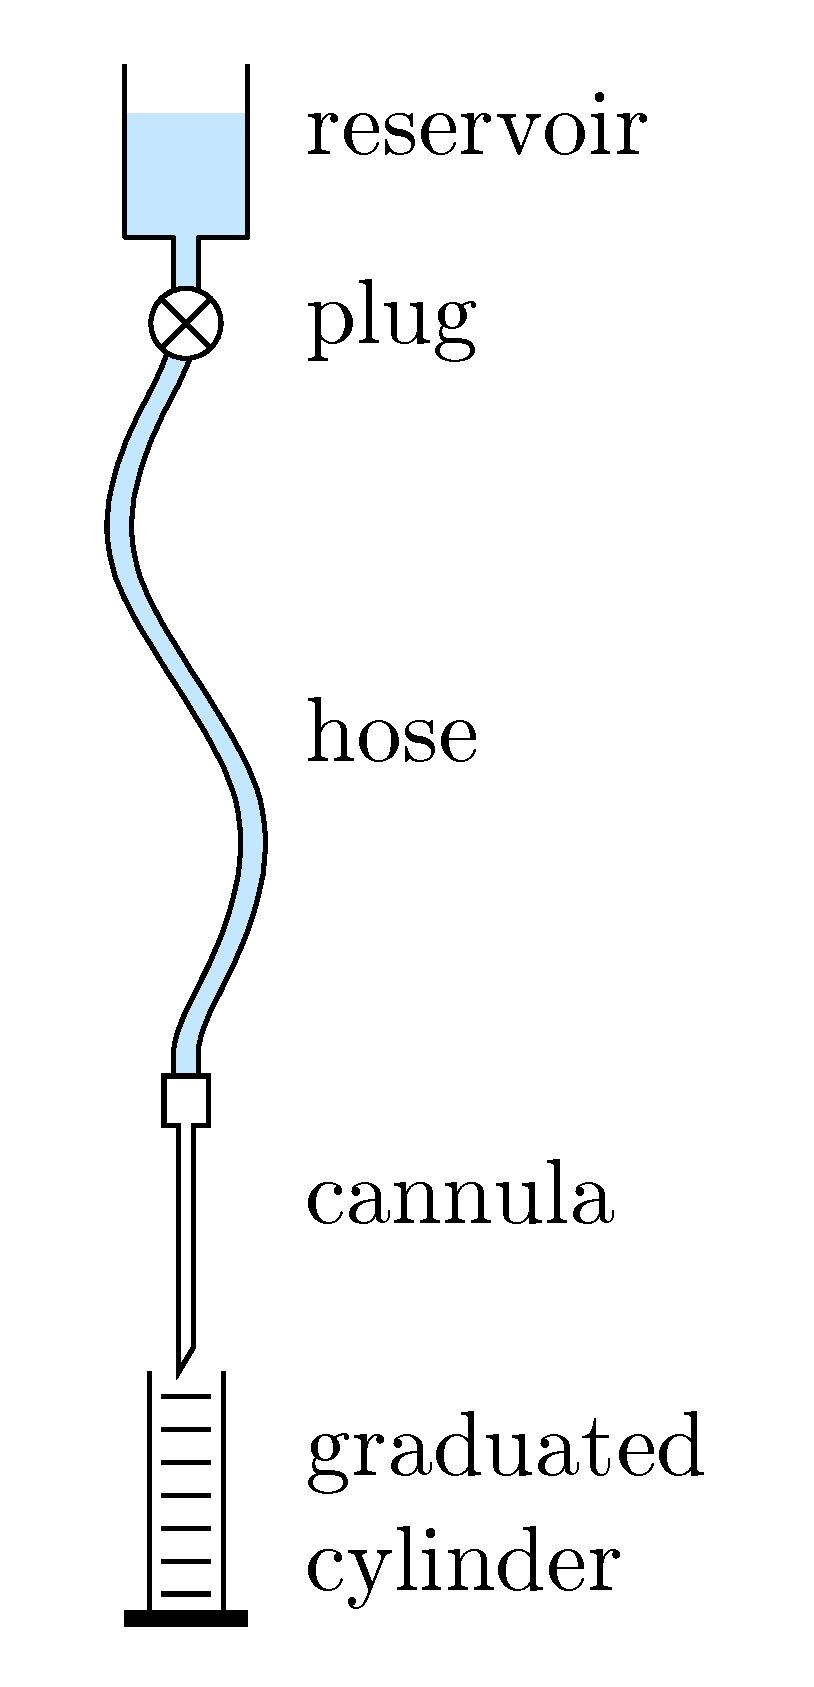
\includegraphics[scale=.25]{Bilder/kanuelen.pdf}
    \caption{capillary viscometer}
    \label{fig:cap}
    \end{minipage}
    \hspace{5mm}
    \begin{minipage}{.3\textwidth}
    \centering
    \vspace{-.2mm}
    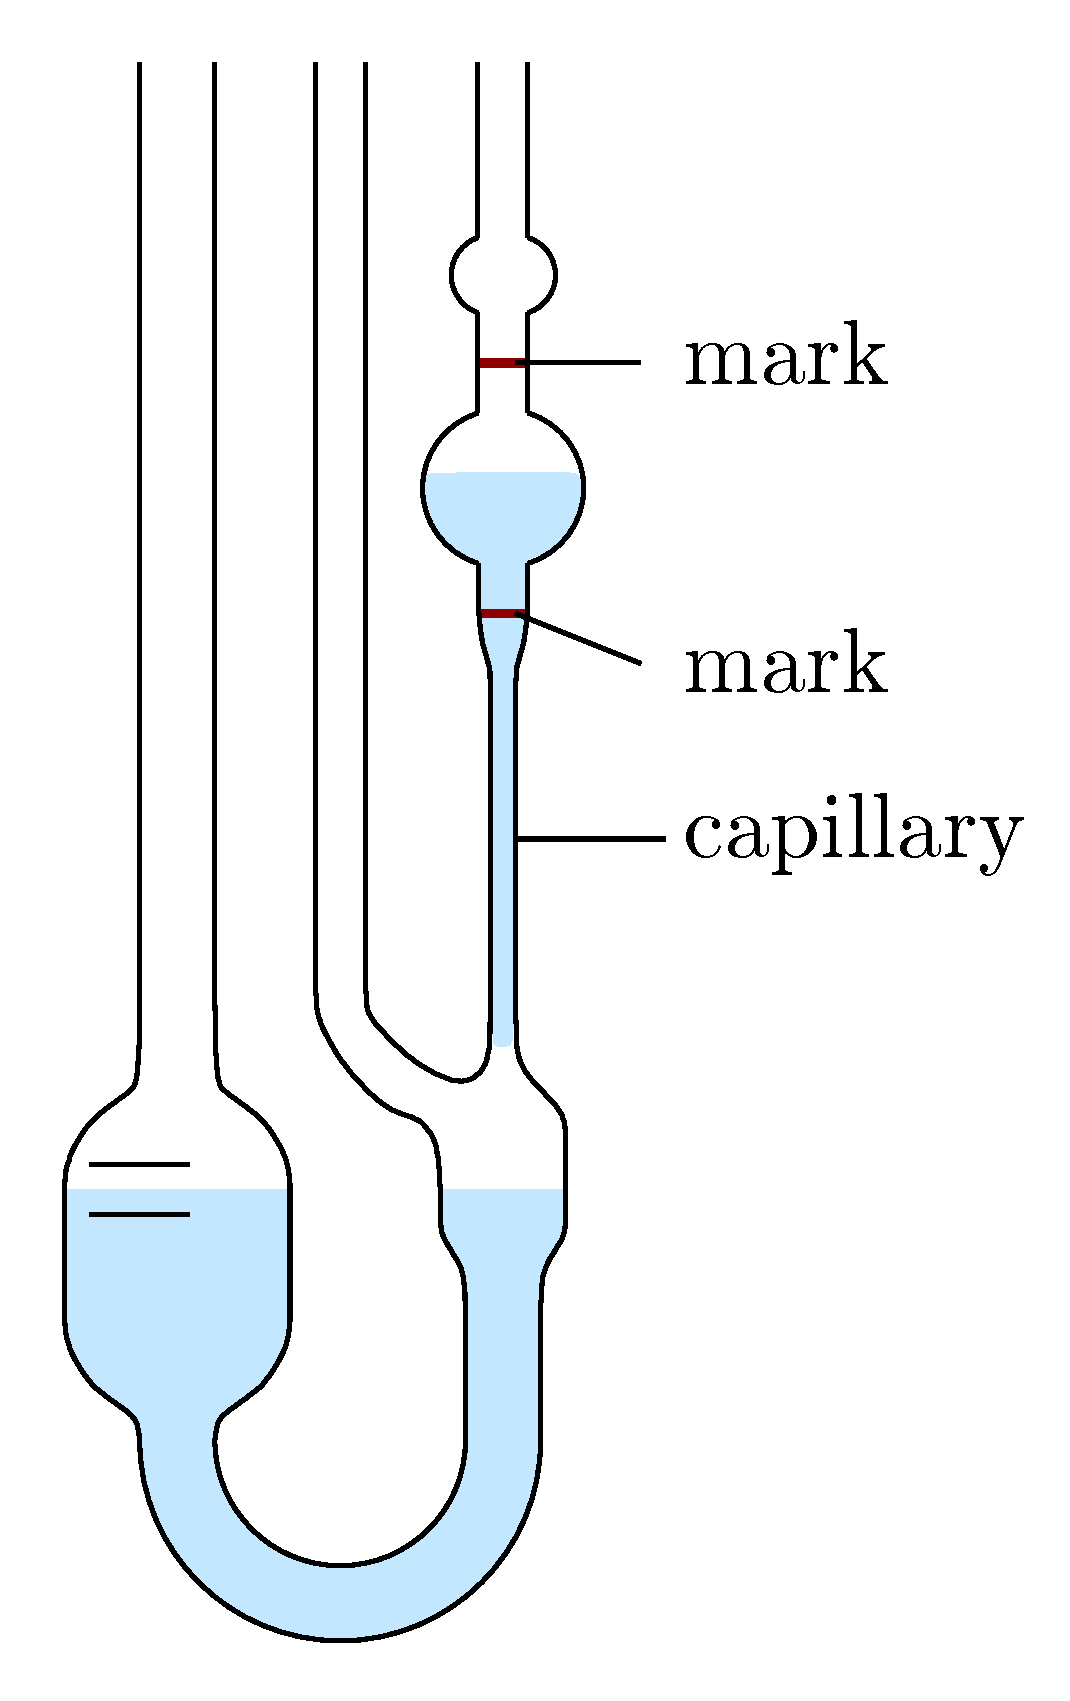
\includegraphics[scale=.25]{Bilder/fancy.pdf}
    \vspace{-.2mm}
    \caption{Ubbelohde viscometer}
    \label{fig:ubb}
    \end{minipage}
\end{figure}